\documentclass[12pt]{article}

\usepackage[margin=2cm]{geometry}
\usepackage[T2A]{fontenc}
\usepackage[utf8]{inputenc}
\usepackage[russian]{babel}
\usepackage{multicol}
\usepackage{longtable}
\usepackage{graphics}
\usepackage{rotating}
\usepackage{float}

\setlength{\parindent}{0em}
\setlength{\parskip}{1em}

\usepackage{amsmath, amsfonts, amssymb, amsthm, mathtools}
\usepackage{icomma}

\title{Отчет о выполнении лабораторной работы \\ Измерение коэффициента поверхностного натяжения воды}
\author{Лепарский Роман}
\date{\today}

\begin{document}

\maketitle

\newpage

\section{Аннотация}

\textbf{Цель работы:} 1) измерение коэффициента поверхностного натяжения исследуемой жидкости при разной температуре с использованием известного коэффициента поверхностного натяжения другой жидкости; 2) определение полной поверхностной энергии и теплоты, необходимой для изотермического образования единицы поверхности жидкости.

\section{Теоретические сведения}

Наличие поверхностного слоя приводит к различию давлений по разные стороны от искривленной границы раздела двух сред. Для сферического пузырька внутри жидкости избыточное давление дается формулой Лапласа:
\begin{equation}
\Delta p = \frac{2\sigma}{r}
\end{equation}

Эта формула лежит в основе предлагаемого метода определения коэффициента поверхностного натяжения жидкости. Измеряется давление, необходимое для выталкивания в жидкость пузырька газа.

\section{Экспериментальная установка}

\begin{figure}[H]
	\centering
	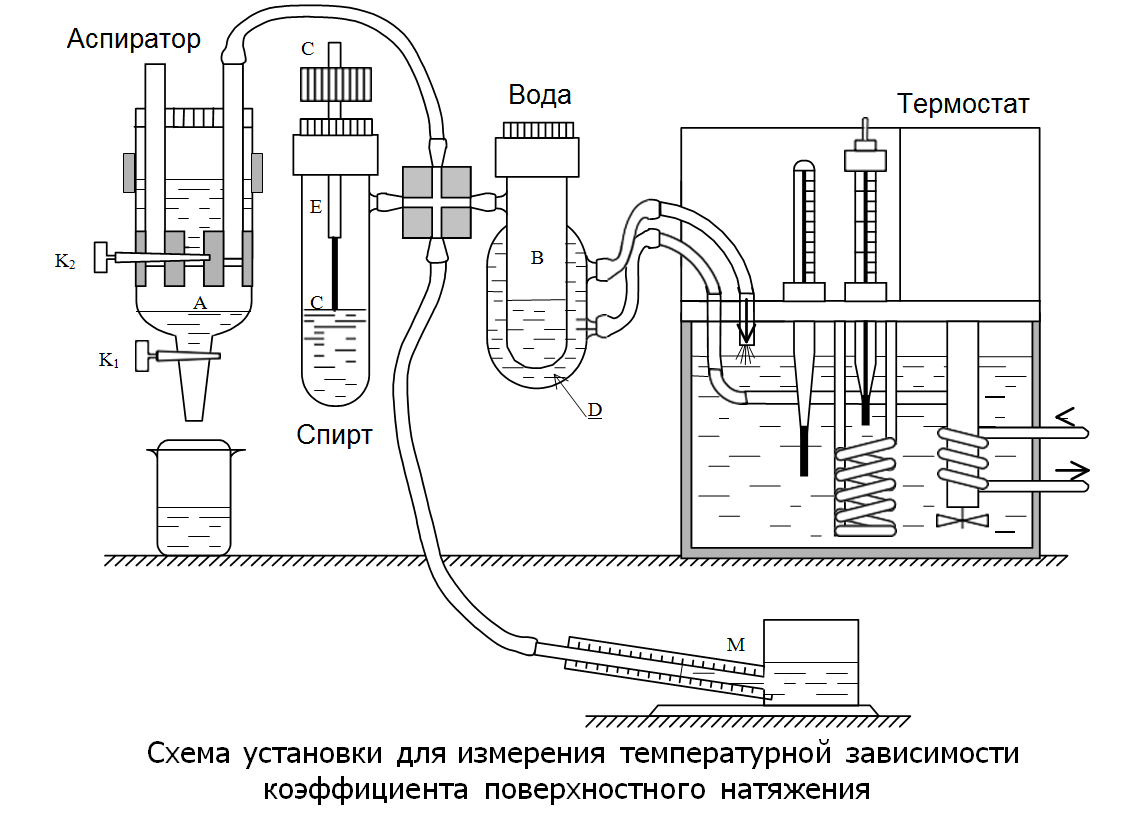
\includegraphics[scale = 0.5]{./images/stand.png}
	\caption{Схема установки}
	\label{fig:stand}
\end{figure}

В резервуар B заливают исследуемую жидкость. Измерения производятся сначала для спирта, чтобы найти радиус пузырька, потом для воды, чтобы определить ее коэффициент поверхностного натяжения воды.

\section{Приборы и материалы}

В работе используются:

\begin{itemize}
	\item прибор Ребиндера с термостатом;
	\item исследуемые жидкости;
	\item стаканы.
\end{itemize}

\section{Обработка результатов}

Запишем результаты измерений для спирта:

\begin{align*}
	\Delta P = 88,2 \pm 0,9 \text{ Па}\\
	\sigma_\text{с} = 0,0223 \text{ Н/м}
\end{align*}

Отсюда, по формуле (1) найдем радиус иглы:
\begin{equation*}
	r = \frac{2\sigma}{\Delta P} = 0,5056 \pm 0.005 \text{ мм}
\end{equation*}

Это значение совпадает с измеренным под микроскопом (0.5 мм).

Далее будем проводить измерения с водой. Глубина погружения иглы, измеренная напрямую $\Delta h = 4,2$ мм. Давление воды на этой глубине $P_\text{в} = 41,16$ Па. Это значение совпадает с разностью давлений внутри пузырька ($P_1 = 225.4$ Па; $P_2 = 307,7$ Па). 

Измерим зависимость температуры жидкости, от давления в пузырьке. Найдем для каждой температуры коэффициент $\sigma$.

\begin{table}[H]
	\centering
	\begin{tabular}{|l|l|l|}
		\hline
		$T$, K & $P$, Па & $\sigma$, Н/м \\ \hline
		298    & 305,76  & 0,0764       \\ \hline
		303    & 301,84  & 0,0754       \\ \hline
		308    & 299,88  & 0,0749       \\ \hline
		313    & 297,92  & 0,0744       \\ \hline
		318    & 294     & 0,0735       \\ \hline
		323    & 292,04  & 0,0730       \\ \hline
		328    & 288,12  & 0,0720       \\ \hline
		333    & 286,16  & 0,0715       \\ \hline
	\end{tabular}
\end{table} 

Рассчитаем по классической формуле погрешность:
\begin{equation*}
	\sigma_\sigma = 0,0002 \text{ Н/м}
\end{equation*}

Построим по данным значениям график $\sigma(T)$

\begin{figure}[H]
	\centering
	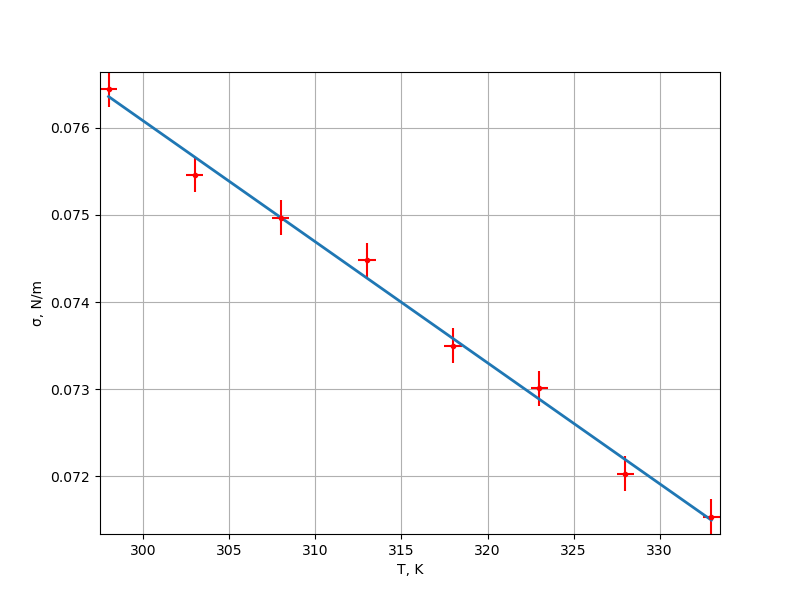
\includegraphics[scale=0.7]{./images/sigma.png}
\end{figure}

Из этого графика находим коэффициент наклона:
\begin{equation*}
	\frac{d\sigma}{dT} = - (138 \pm 4) \cdot 10^{-6} \text{ Н/м*К}
\end{equation*}

С помощью него найдем следующие величины:
\begin{align*}
	q &= -T\frac{d\sigma}{dT}\\
	\frac{Q_\Pi}{\Pi} &=\sigma - T\frac{d\sigma}{dT}
\end{align*}

Запишем результаты в таблицу:
\begin{table}[H]
	\centering
	\begin{tabular}{|l|l|l|}
		\hline
		$T$, K & $q$, Н/м          & $Q/\Pi$, Н/м      \\ \hline
		298    & 0,0413 & 0,0350 \\ \hline
		303    & 0,0420 & 0,0333 \\ \hline
		308    & 0,0427 & 0,0322 \\ \hline
		313    & 0,0434 & 0,0310 \\ \hline
		318    & 0,0441 & 0,0293 \\ \hline
		323    & 0,0448 & 0,0281 \\ \hline
		328    & 0,0455 & 0,0264 \\ \hline
		333    & 0,0462 & 0,0253 \\ \hline
	\end{tabular}
\end{table}

Найдем погрешности:
\begin{align*}
	\sigma_q = 0,0006 \text{ Н/м}\\
	\sigma_{Q/\Pi} = 0,0006 \text{ Н/м}
\end{align*}

Построим графики по найденным значениям:
\begin{figure}[H]
	\centering
	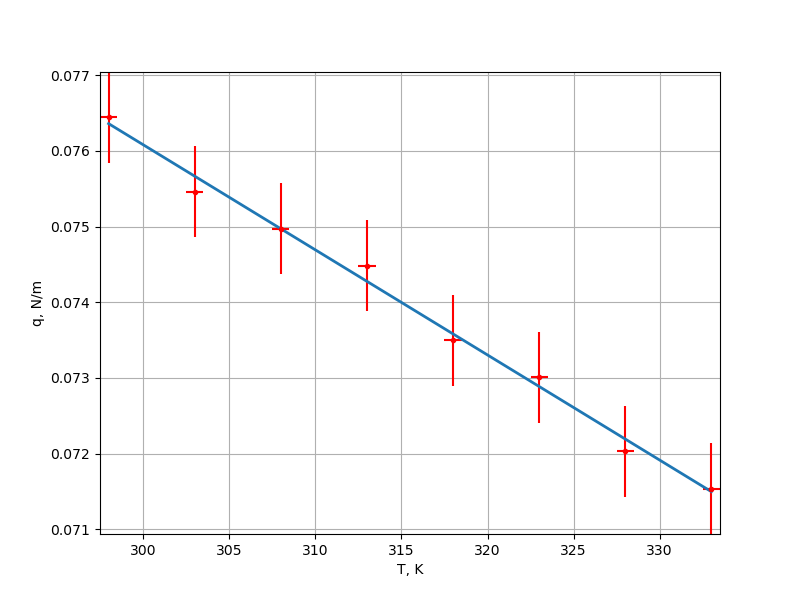
\includegraphics[scale=0.7]{./images/q.png}
\end{figure}

\begin{figure}[H]
	\centering
	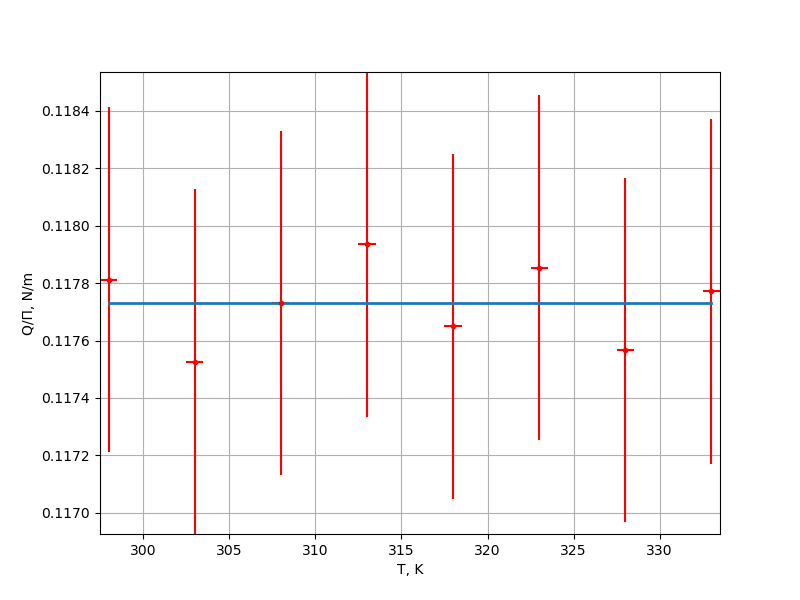
\includegraphics[scale=0.7]{./images/Qp.png}
\end{figure}

\section{Вывод}

С помощью уравнения Лапласа нам удалось найти радиус иглы $r= 0,5056 \pm 0.005  \text{ мм}$, причем, с большей точностью по сравнению с прямым измерением. Также удалось определить коэффициент поверхностного натяжения воды $\sigma = 0,0764 \pm 0.0002$ Н/м (t = 25 $^\circ C$) и его зависимость от температуры $\frac{d\sigma}{dT} = - (138 \pm 4) \cdot 10^{-6} \text{ Н/м*К}$. Эти значения лежат близко к табличным ($\sigma = 0,073$ Н/м; $\frac{d\sigma}{dT} = - 168 \cdot 10^{-6} \text{ Н/м*К}$). Допустимость аппроксимации зависимости $\sigma(T)$ прямой подтверждается последним графиком.

\end{document}